\section{Changing the Start Vectors} \label{sec:changing_start_vectors}

The one obviously suboptimal choice regarding the parameters of the baseline case is to start by placing every cell uniformly random on the chip area.
It can be easily seen from \cref{fig:baseline_objective_function_convergence_by_gamma} that the wirelength of this placement
is higher than optimum by several orders of magnitude.
It could improve the results and also decrease the number of iterations needed
to start with a placement that has a lower weighted wirelength (measured with HPWL)
because presumably such a placement is also closer to the optimum.
Let us start by placing all cells at the center of the chip at the beginning of the optimization.
All remaining parameters stay the same as before.

\begin{figure}[t]
 \centering

 \begin{subfigure}{.48\textwidth}
  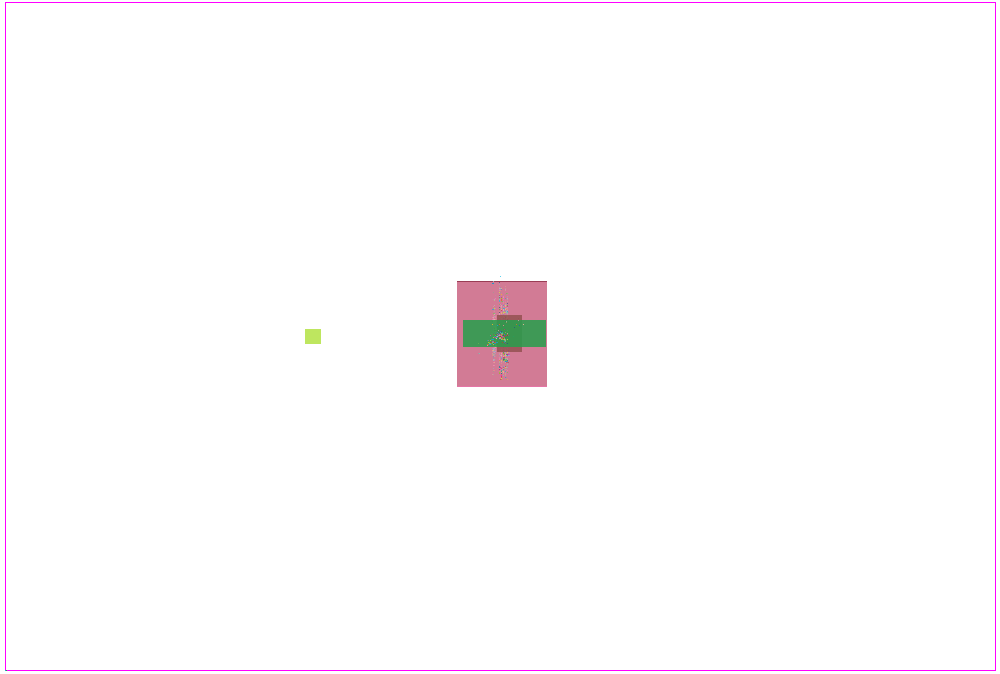
\includegraphics[width=\textwidth]{start_vectors/convergence_Chip1_LSE_center_1000_gamma.png}  
  \caption{\(T_{\NLSE_\gamma}\) with \(\gamma = 10^3\)}
 \end{subfigure}
 \hfill
 \begin{subfigure}{.48\textwidth}
  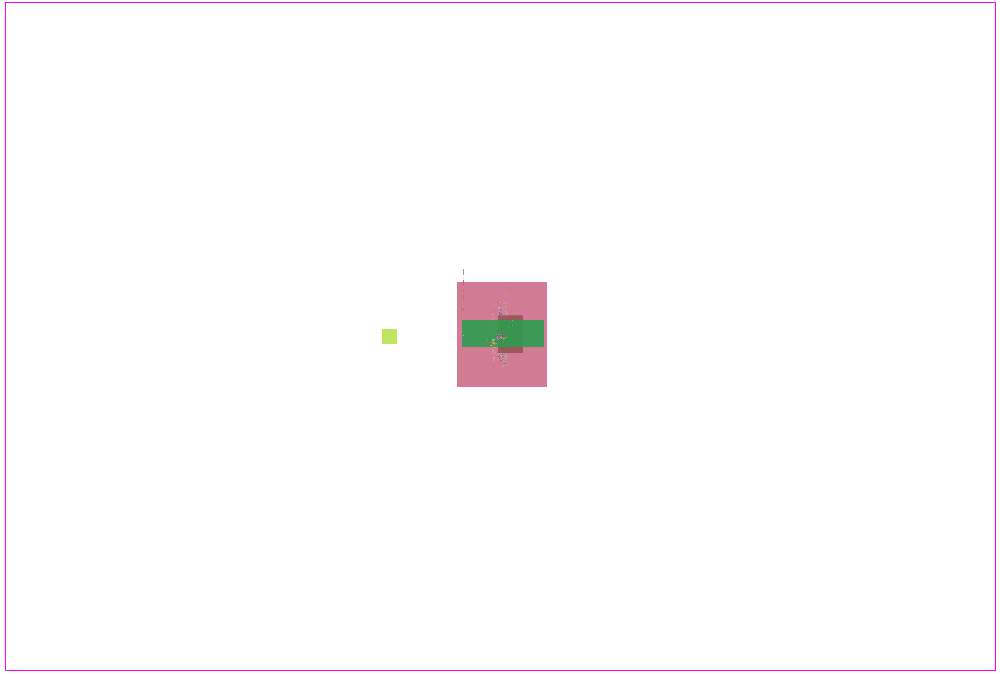
\includegraphics[width=\textwidth]{start_vectors/convergence_Chip1_WA_center_1000_gamma.png}  
  \caption{\(T_{\NWA_\gamma}\) with \(\gamma = 10^3\)}
 \end{subfigure}
 
 \bigskip
 
 \begin{subfigure}{.48\textwidth}
  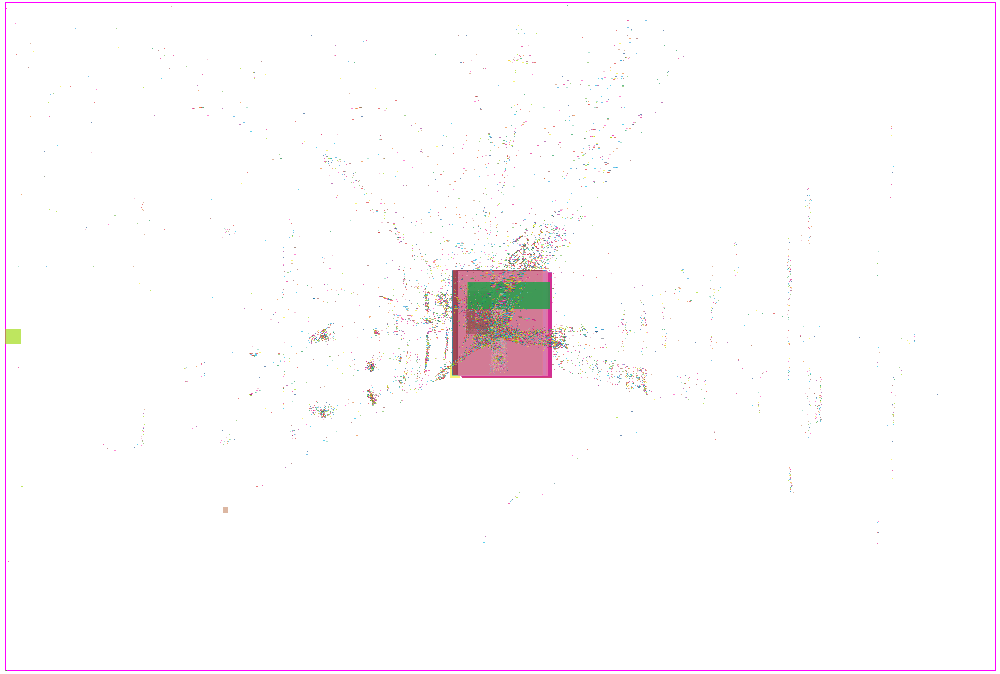
\includegraphics[width=\textwidth]{start_vectors/convergence_Chip1_LSE_center_100000_gamma.png}  
  \caption{\(T_{\NLSE_\gamma}\) with \(\gamma = 10^5\)}
 \end{subfigure}
 \hfill
 \begin{subfigure}{.48\textwidth}
  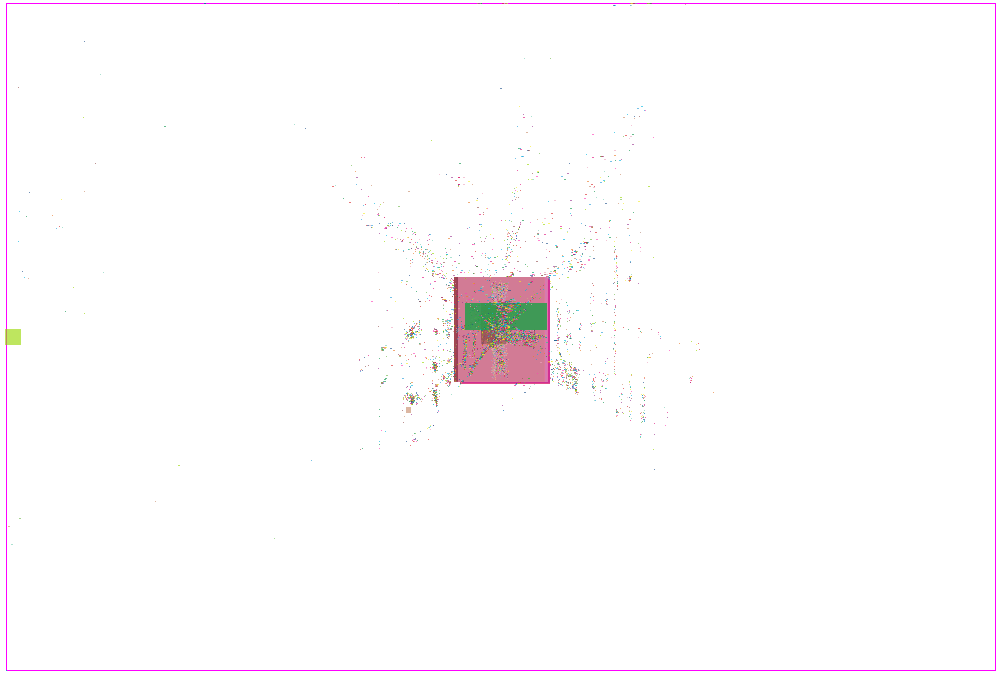
\includegraphics[width=\textwidth]{start_vectors/convergence_Chip1_WA_center_100000_gamma.png}  
  \caption{\(T_{\NWA_\gamma}\) with \(\gamma = 10^5\)}
 \end{subfigure}
 
 \caption{Placement plots after 1000 NAG iterations using the specified objective function}
 \label{fig:center_placement_plots}
\end{figure}

% TODO: Put movement plots for \gamma = 10^3 directly below and change the placement specifier to p

We can skip the graphs for the objective function and gradient norms during the optimization process
and directly look at the resulting placements
because they show a serious problem.
In \cref{fig:center_placement_plots}, the placements after 1000 NAG iterations are shown
for both \(T_{\NLSE_\gamma}\) and \(T_{\NWA_\gamma}\) and \(\gamma \in \{10^3, 10^5\}\)
(the plot for \(\gamma = 10^1\) is extremely similar to the one with \(\gamma = 10^3\)).
The parameter \(\gamma\) controls the smoothness for both approximations of \(\HPWL\).
When decreasing \(\gamma\), the smoothness decreases and 
\texttt{backtracking-line-search} has to reduce the step size more.
For \(\gamma = 10^3\) the step size is decreased so much that the cells barely move and 
even after 1000 iterations none of the cells are at one of the edges of the chip.
Even though the objective function and \(\HPWL\) are better
than using a random initial placement,
the placements are useless in guiding a partitioning process.
Therefore, the rest of this section will only investigate the impact of different
start vectors with respect to \(\gamma = 10^5\).

The details about the different start vectors can be found in \cref{subsec:implementation_start_vector}.
In summary, the parameters used for this section are
\begin{itemize}
 \item Objective function: \(T_{\NLSE_\gamma}\) or \(T_{\NWA_\gamma}\) with \(\gamma = 10^5\)
 \item Start vector: RANDOM, CENTER, HPWL-OPT or QCLIQUE-OPT
 \item Optimization method: Nesterov's accelerated gradient method
 \item The step size strategy: \texttt{backtracking-line-search}
 \item The stop criterion: After exactly 1000 iterations
\end{itemize}

\begin{figure}[t]
 \centering
 \begin{tikzpicture}
  \begin{groupplot} [
      width=(\textwidth-1cm),
      height=(\textwidth-1cm)/2,
      group style={group size=1 by 2},
      group/xlabels at=edge bottom,
      xlabel=Iteration,
      enlarge x limits={value=0.05, upper},
      y unit=\si{\meter},
  ]
   \nextgroupplot[
       ylabel=\(T_{\NLSE_\gamma}\),
       ymax=180.75,
       restrict y to domain=178:181
   ]
   
   \addlegendentry{RANDOM}
   \addplot [red, thick] table [
     x=iteration,
     y=LSE_random_100000_gamma_objective,
   ] {chapters/results/start_vectors/convergence_Chip1_100000_gamma.data};
   
   \addlegendentry{CENTER}
   \addplot [dark_green, thick] table [
     x=iteration,
     y=LSE_center_100000_gamma_objective,
   ] {chapters/results/start_vectors/convergence_Chip1_100000_gamma.data};

   \addlegendentry{QCLIQUE-OPT}
   \addplot [blue, thick] table [
     x=iteration,
     y=LSE_qp_100000_gamma_objective,
   ] {chapters/results/start_vectors/convergence_Chip1_100000_gamma.data};

   \addlegendentry{HPWL-OPT}
   \addplot [Goldenrod, thick] table [
     x=iteration,
     y=LSE_hpwl_100000_gamma_objective,
   ] {chapters/results/start_vectors/convergence_Chip1_100000_gamma.data};

   \nextgroupplot[
       ylabel=\(T_{\NWA_\gamma}\),
       ymax=4.8,
       restrict y to domain=2:6
   ]
   
   \addlegendentry{RANDOM}
   \addplot [red, thick] table [
     x=iteration,
     y=WA_random_100000_gamma_objective,
   ] {chapters/results/start_vectors/convergence_Chip1_100000_gamma.data};
   
   \addlegendentry{CENTER}
   \addplot [dark_green, thick] table [
     x=iteration,
     y=WA_center_100000_gamma_objective,
   ] {chapters/results/start_vectors/convergence_Chip1_100000_gamma.data};

   \addlegendentry{QCLIQUE-OPT}
   \addplot [blue, thick] table [
     x=iteration,
     y=WA_qp_100000_gamma_objective,
   ] {chapters/results/start_vectors/convergence_Chip1_100000_gamma.data};

   \addlegendentry{HPWL-OPT}
   \addplot [Goldenrod, thick] table [
     x=iteration,
     y=WA_hpwl_100000_gamma_objective,
   ] {chapters/results/start_vectors/convergence_Chip1_100000_gamma.data};
  \end{groupplot}
 \end{tikzpicture}
 \caption{Objective function by iteration depending on start vectors} 
 \label{fig:objective_convergence_by_start_vectors}
\end{figure}

The first observation is that the hope at the start of this section was justified:
By not using a random initial placement, the objective function is indeed lower during the whole optimization process.
This is true for CENTER and the effect increases when starting with QCLIQUE-OPT or HPWL-OPT as start vectors
as shown in \cref{fig:objective_convergence_by_start_vectors}.
This was expected as the latter two options already incorporate netlist information.
Interestingly, the \(T_{\NLSE_\gamma}\) is minimal when using QCLIQUE-OPT
and \(T_{\NWA_\gamma}\) is minimal when using HPWL-OPT
which is another indicator that \(\NWA_\gamma\) better correlates with \(\HPWL\) than \(\NLSE_\gamma\).

\begin{sidewaysfigure}[p]
 \centering

 \begin{subfigure}{.32\textwidth}
  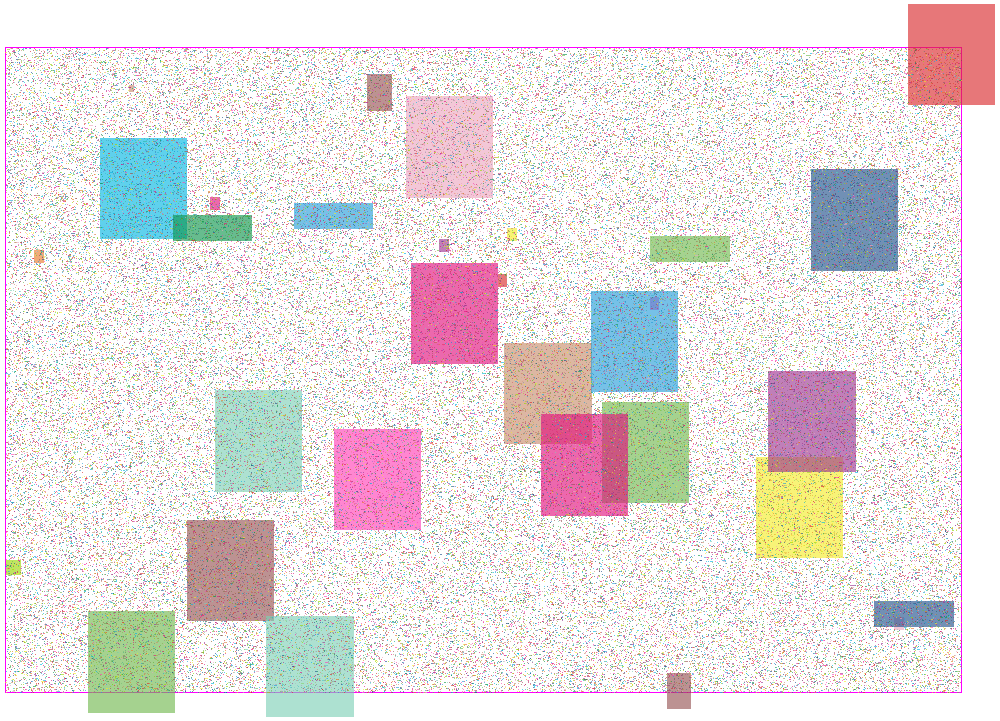
\includegraphics[width=\textwidth]{start_vectors/convergence_Chip1_random.png}  
  \caption{RANDOM}
 \end{subfigure}
 \hfill
 \begin{subfigure}{.32\textwidth}
  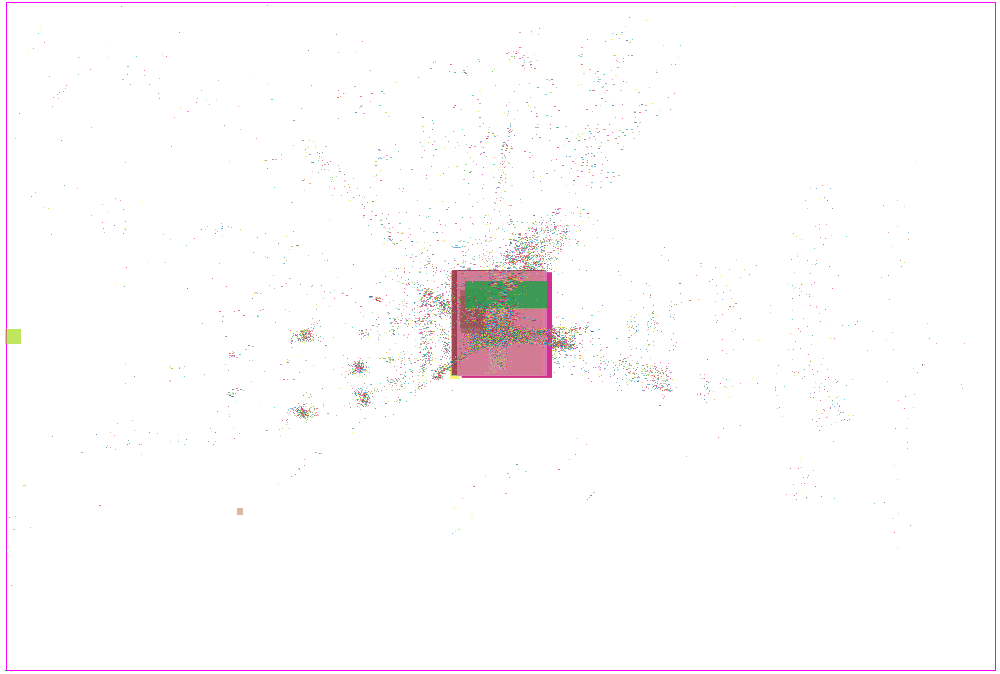
\includegraphics[width=\textwidth]{start_vectors/convergence_Chip1_LSE_random_100000_gamma.png}  
  \caption{\(T_{\NLSE_\gamma}\) with \(\gamma = 10^5\)}
 \end{subfigure}
 \hfill
 \begin{subfigure}{.32\textwidth}
  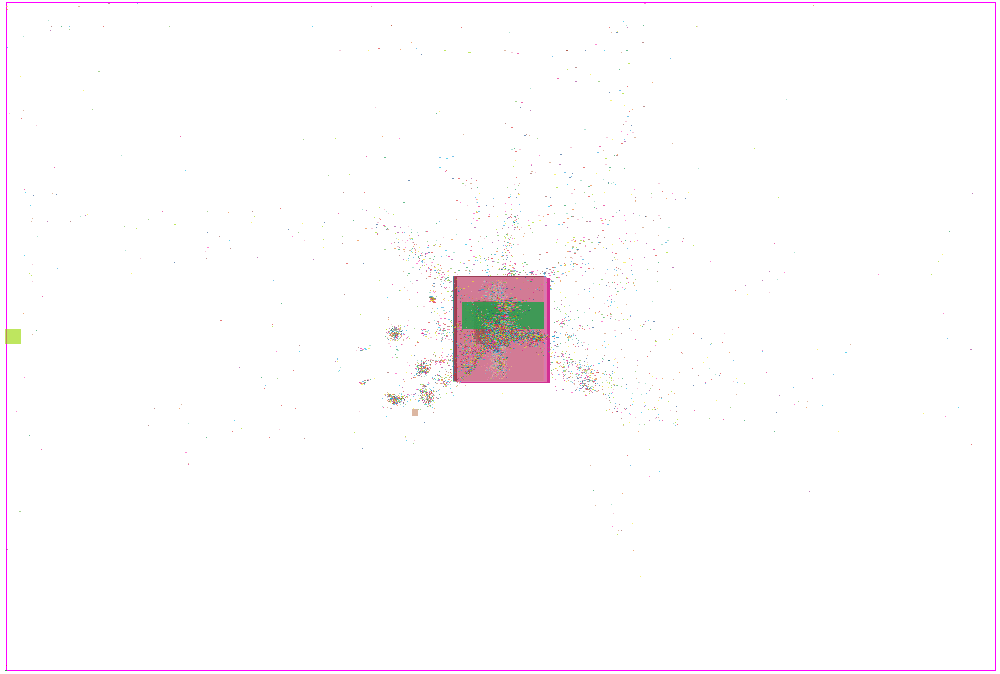
\includegraphics[width=\textwidth]{start_vectors/convergence_Chip1_WA_random_100000_gamma.png}  
  \caption{\(T_{\NWA_\gamma}\) with \(\gamma = 10^5\)}
 \end{subfigure}

 \bigskip
 
 \begin{subfigure}{.32\textwidth}
  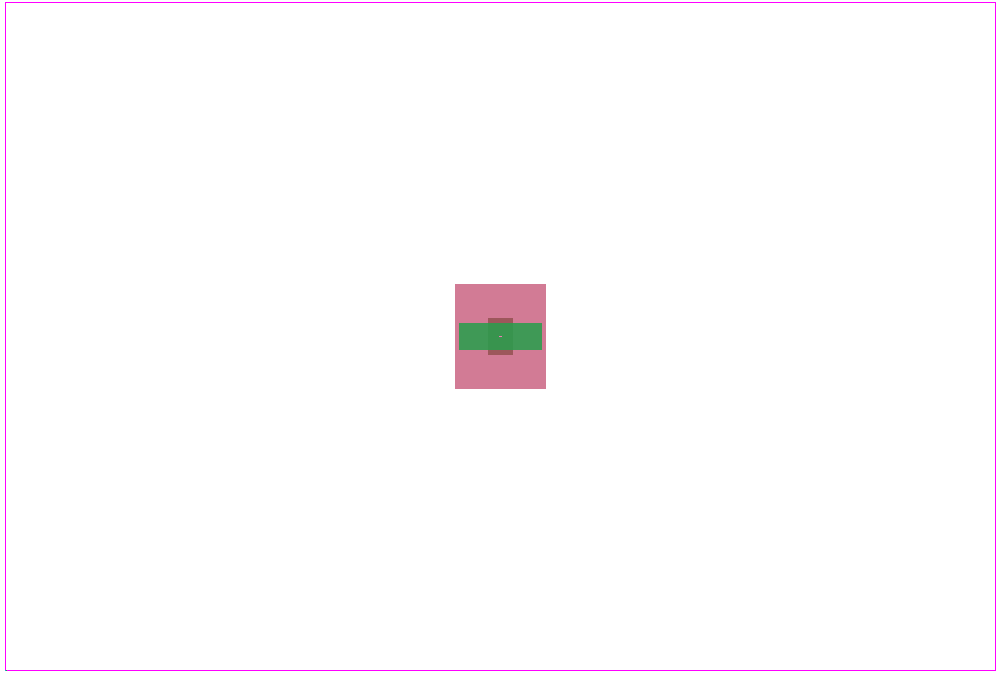
\includegraphics[width=\textwidth]{start_vectors/convergence_Chip1_center.png}  
  \caption{CENTER}
 \end{subfigure}
 \hfill
 \begin{subfigure}{.32\textwidth}
  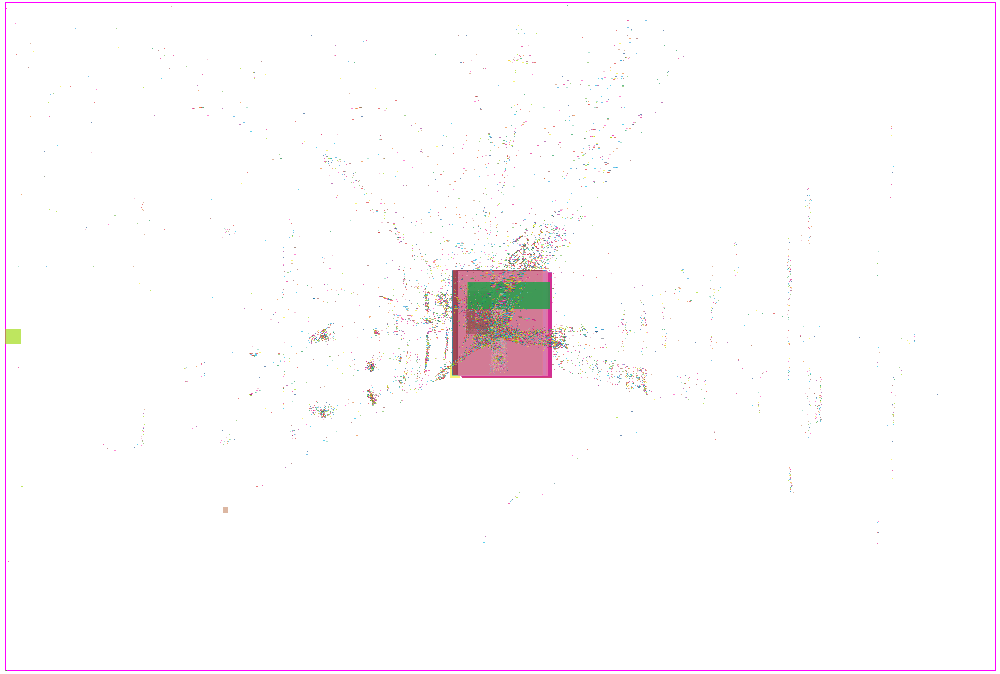
\includegraphics[width=\textwidth]{start_vectors/convergence_Chip1_LSE_center_100000_gamma.png}  
  \caption{\(T_{\NLSE_\gamma}\) with \(\gamma = 10^5\)}
 \end{subfigure}
 \hfill
 \begin{subfigure}{.32\textwidth}
  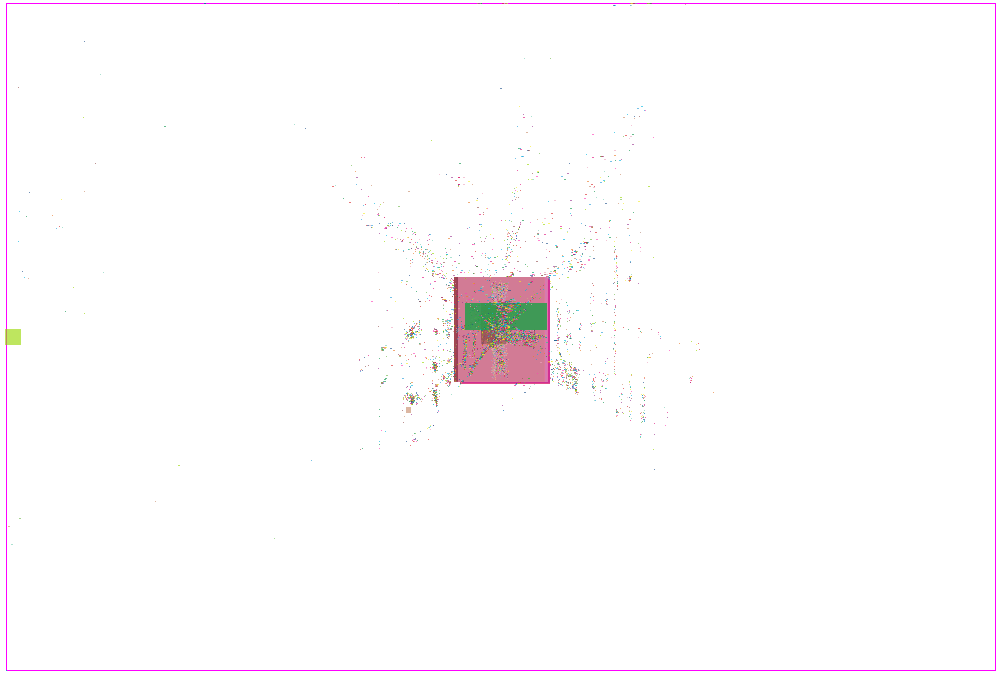
\includegraphics[width=\textwidth]{start_vectors/convergence_Chip1_WA_center_100000_gamma.png}  
  \caption{\(T_{\NWA_\gamma}\) with \(\gamma = 10^5\)}
 \end{subfigure}

 \caption{Placement plots after 1000 NAG iterations using the specified objective function.
          The start vector is the same as at the leftmost image.}
 \label{fig:start_vectors_placement_plots}
\end{sidewaysfigure}
\begin{sidewaysfigure}[p]\ContinuedFloat
 \centering
 \begin{subfigure}{.32\textwidth}
  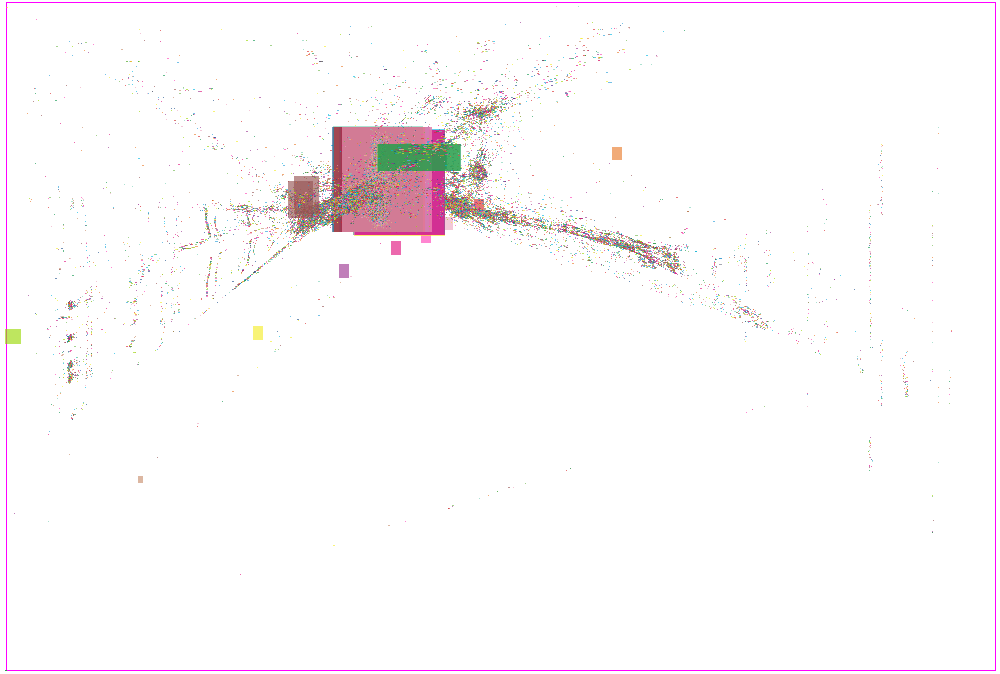
\includegraphics[width=\textwidth]{start_vectors/convergence_Chip1_qp.png}  
  \caption{QCLIQUE-OPT}
 \end{subfigure}
 \hfill
 \begin{subfigure}{.32\textwidth}
  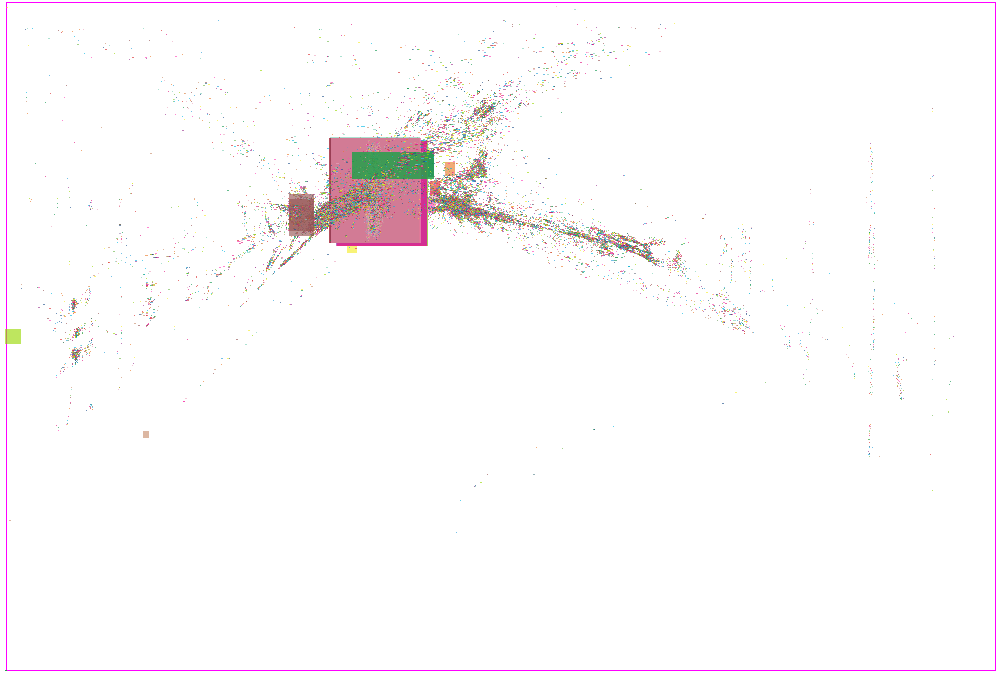
\includegraphics[width=\textwidth]{start_vectors/convergence_Chip1_LSE_qp_100000_gamma.png}  
  \caption{\(T_{\NLSE_\gamma}\) with \(\gamma = 10^5\)}
 \end{subfigure}
 \hfill
 \begin{subfigure}{.32\textwidth}
  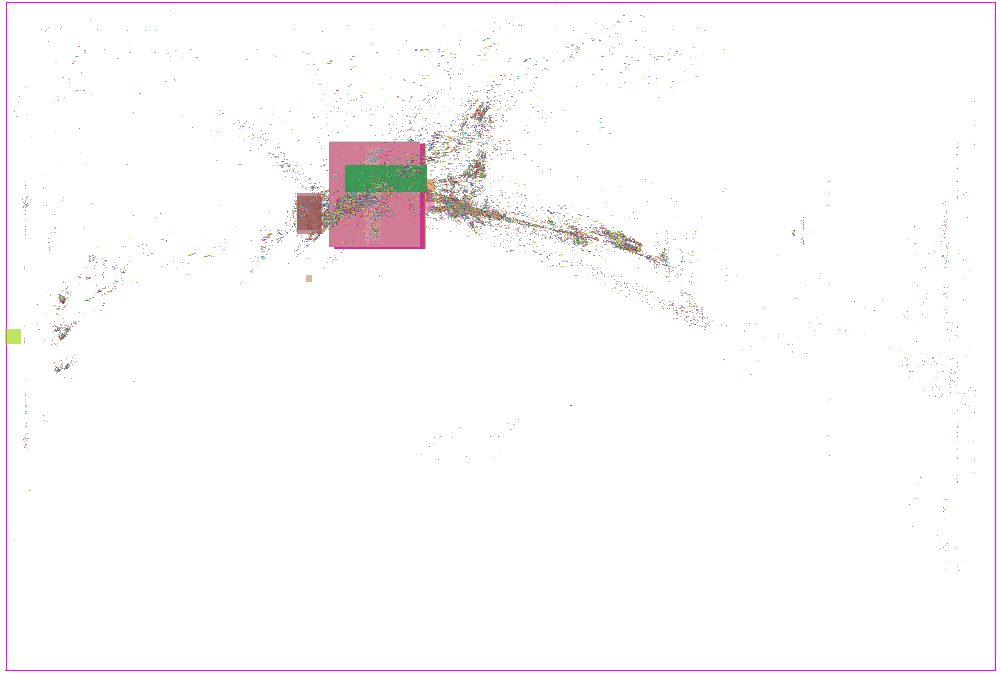
\includegraphics[width=\textwidth]{start_vectors/convergence_Chip1_WA_qp_100000_gamma.png}  
  \caption{\(T_{\NWA_\gamma}\) with \(\gamma = 10^5\)}
 \end{subfigure}

 \bigskip
 
 \begin{subfigure}{.32\textwidth}
  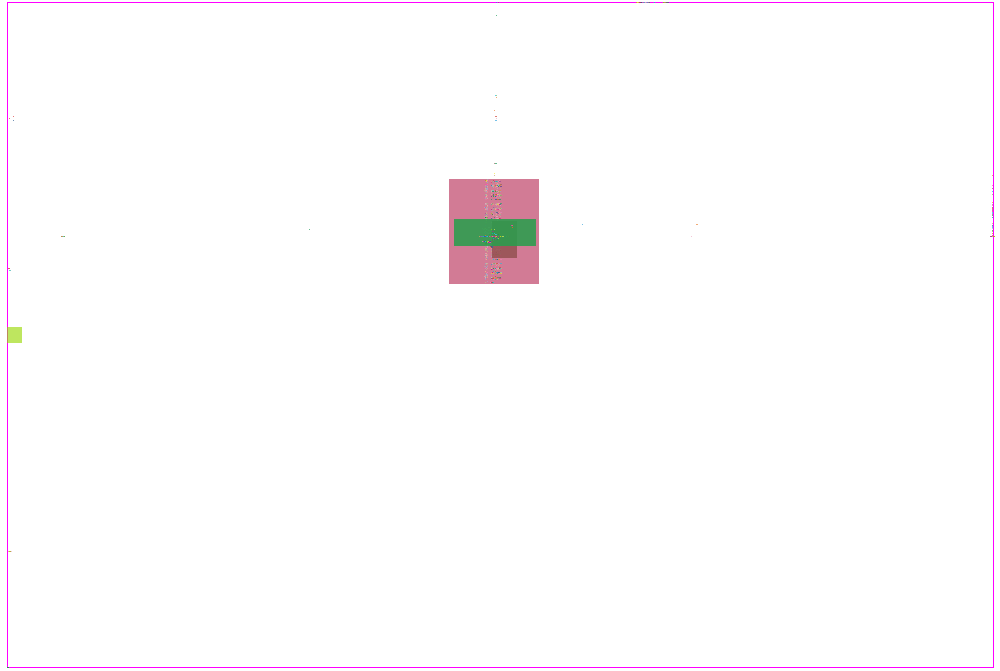
\includegraphics[width=\textwidth]{start_vectors/convergence_Chip1_hpwl.png}  
  \caption{HPWL-OPT}
 \end{subfigure}
 \hfill
 \begin{subfigure}{.32\textwidth}
  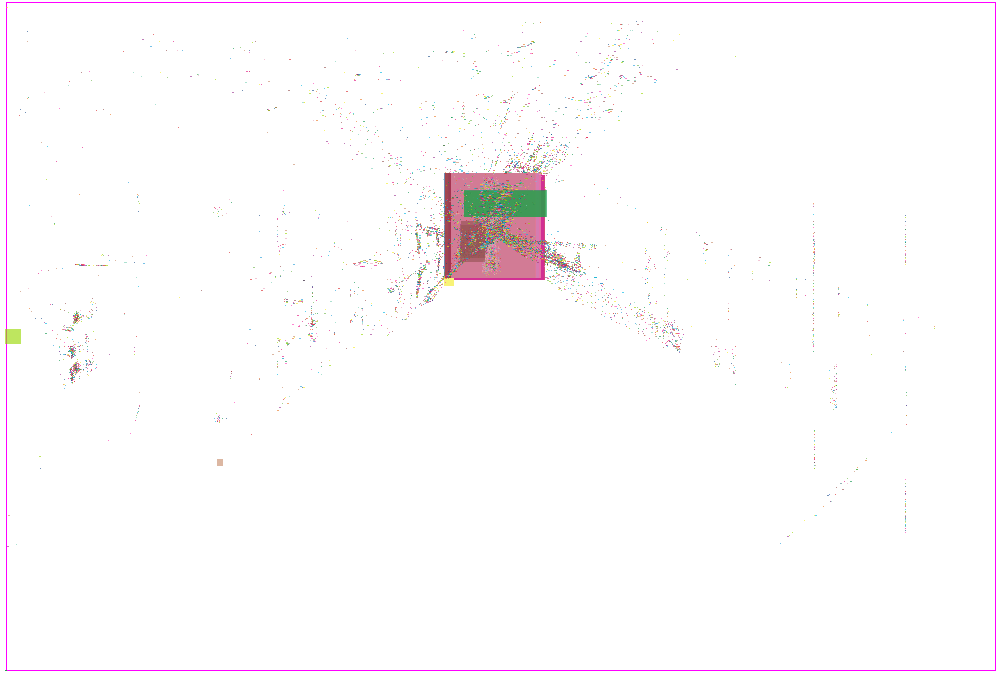
\includegraphics[width=\textwidth]{start_vectors/convergence_Chip1_LSE_hpwl_100000_gamma.png}  
  \caption{\(T_{\NLSE_\gamma}\) with \(\gamma = 10^5\)}
 \end{subfigure}
 \hfill
 \begin{subfigure}{.32\textwidth}
  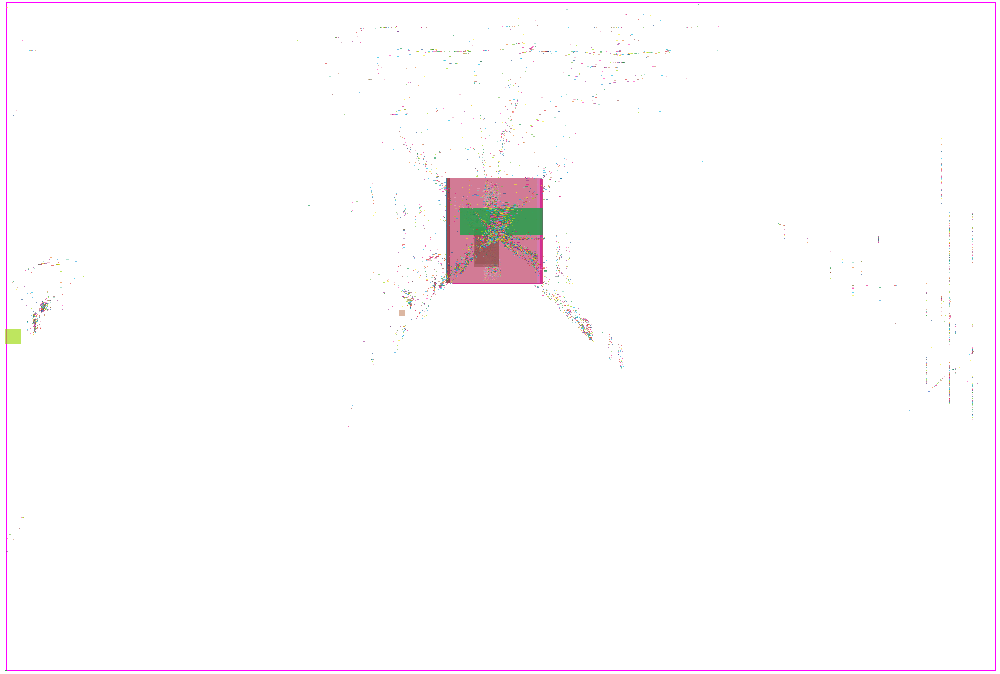
\includegraphics[width=\textwidth]{start_vectors/convergence_Chip1_WA_hpwl_100000_gamma.png}  
  \caption{\(T_{\NWA_\gamma}\) with \(\gamma = 10^5\)}
 \end{subfigure}

 \caption{Placement plots after 1000 NAG iterations using the specified objective function.
          The start vector is the same as at the leftmost image.}
\end{sidewaysfigure}

\Cref{fig:start_vectors_placement_plots} shows that the final placement using CENTER
is similar to the one starting with random cell positions,
so CENTER achieves much better results during the early iterations and similar ones at the end
which makes it the overall better initial placement.
Simultaneously, the final placements after starting with CENTER, QCLIQUE-OPT and HPWL-OPT
are very different even though \cref{fig:objective_convergence_by_start_vectors} shows
that they have similarly low values of the objective functions.
Therefore, the \enquote{valley} of optimal placements with respect to \(T_{\NLSE_\gamma}\) and \(T_{\NWA_\gamma}\)
has to be very flat for higher values of \(\gamma\).
While the objective function converges to its minimum
regardless of the direction that the valley is approached from,
the final placement can wildly differ and in particular
the weighted wirelength using \(\HPWL\) can have very different values.

\begin{figure}[t]
 \centering
 \begin{tikzpicture}
  \begin{axis} [
      width=(\textwidth-4.5cm),
      height=(\textwidth-1cm)/2,
      ybar,
      ylabel=\(T_{\HPWL}\),
      y unit=\si{\meter},
      ymin=0,
      symbolic x coords={NLSE,NWA},
      xticklabels={\(T_{\NLSE_\gamma}\),\(T_{\NWA_\gamma}\)},
      xtick=data,
      enlarge x limits=0.7,
      bar width=0.8cm,
      legend pos=outer north east,
  ]
   \addlegendentry{RANDOM}
   \addplot [red, fill=red!50!white] coordinates {
       (NLSE, 9.90477)
       (NWA, 9.04183)
   };
   
   \addlegendentry{CENTER}
   \addplot [dark_green, fill=dark_green!50!white] coordinates {
       (NLSE, 6.463749999999999)
       (NWA, 5.58311)
   };

   \addlegendentry{QCLIQUE-OPT}
   \addplot [blue, fill=blue!50!white] coordinates {
       (NLSE, 7.665940000000001)
       (NWA, 7.0313799999999995)
   };

   \addlegendentry{HPWL-OPT}
   \addplot [Goldenrod, fill=Goldenrod!50!white] coordinates {
       (NLSE, 6.60487)
       (NWA, 5.579269999999999)
   };
   
   \addlegendentry{min \(T_{\HPWL}\)}
   \addlegendimage{black,line legend,sharp plot}
   \coordinate (A) at (axis cs:NLSE,4.020);
   \coordinate (O1) at (rel axis cs:0,0);
   \coordinate (O2) at (rel axis cs:1,0);
   \draw [black,sharp plot] (A -| O1) -- (A -| O2);
  \end{axis}
 \end{tikzpicture}
 \caption{Linear wirelength \(T_{\HPWL}\) of the final placements depending on the start vectors}
 \label{fig:start_vectors_hpwl_comparison}
\end{figure}

To investigate the difference between the values of \(T_{\HPWL}\),
take a look at \cref{fig:start_vectors_hpwl_comparison}.
All of the new methods for choosing the start vectors are improving
the value that was achieved by random start values.
The graph of \(T_{\HPWL}\) during the optimization procedure is not shown here
but it indicates that the value will further decrease with more iterations for QCLIQUE-OPT
while it will increase for CENTER and HPWL-OPT.
Because CENTER performs considerably better than RANDOM
and is much cheaper than the other two methods,
it will be the default for our further investigations.

Summarizing the new insights of this section we can say
that the NLSE and NWA objective functions using \(\gamma < 10^5\) are not smooth enough to be used with NAG,
that the CENTER start vectors clearly lead to faster convergence than RANDOM for the objective functions with \(\gamma = 10^5\)
and that these objective functions become very flat towards their minima
such that very different placements can achieve close to optimal values.
